%!TEX root = ../Pflichtenheft.tex

\chapter{Produktübersicht}



\section{Die Registration}


\begin{figure}[ht]
\centering
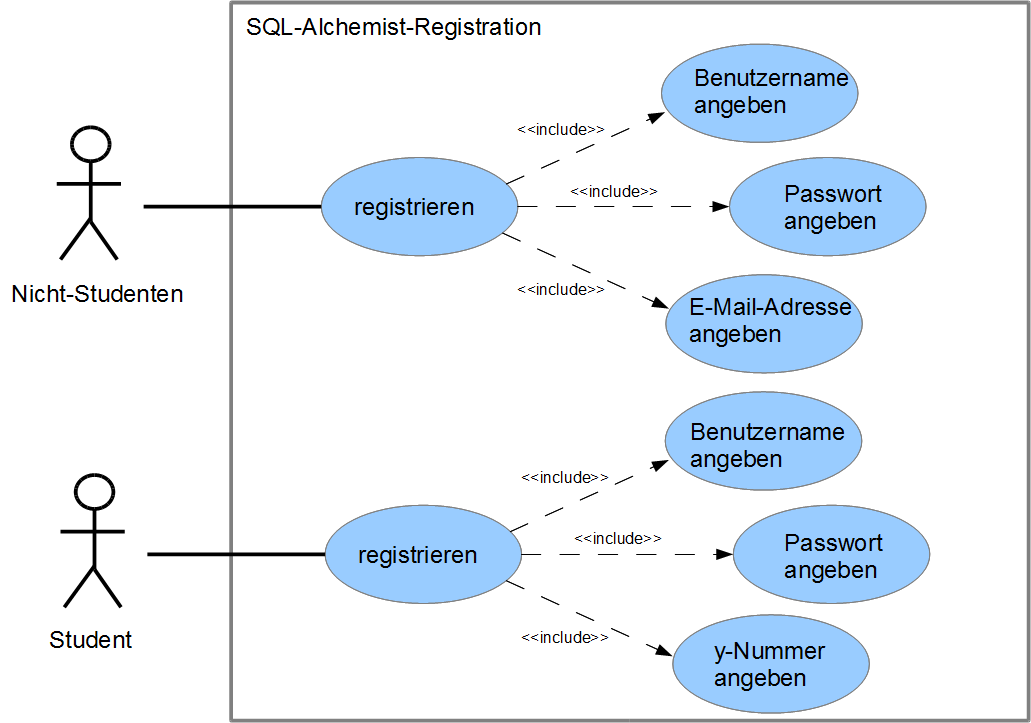
\includegraphics[width=1.0\textwidth]{figures/Registration.PNG}
\caption{Die Registration}
\end{figure}\\
In diesem Use-Case-Diagramm werden die Abl\"aufe aus Nutzersicht beschrieben, die zur Registration nötig sind. Dabei muss zwischen Studenten und Nicht-Studenten unterschieden werden.
Studenten müssen zur Registration ihre y-Nummer, einen Benutzernamen und das zu ihrer y-Nummer gehörige Passwort angeben.\\
Nicht-Student müssen zur Registration eine E-Mail-Adresse, einen Benutzernamen und ein Passwort angeben.\\\\\\\\\\




\begin{figure}[ht]
\centering
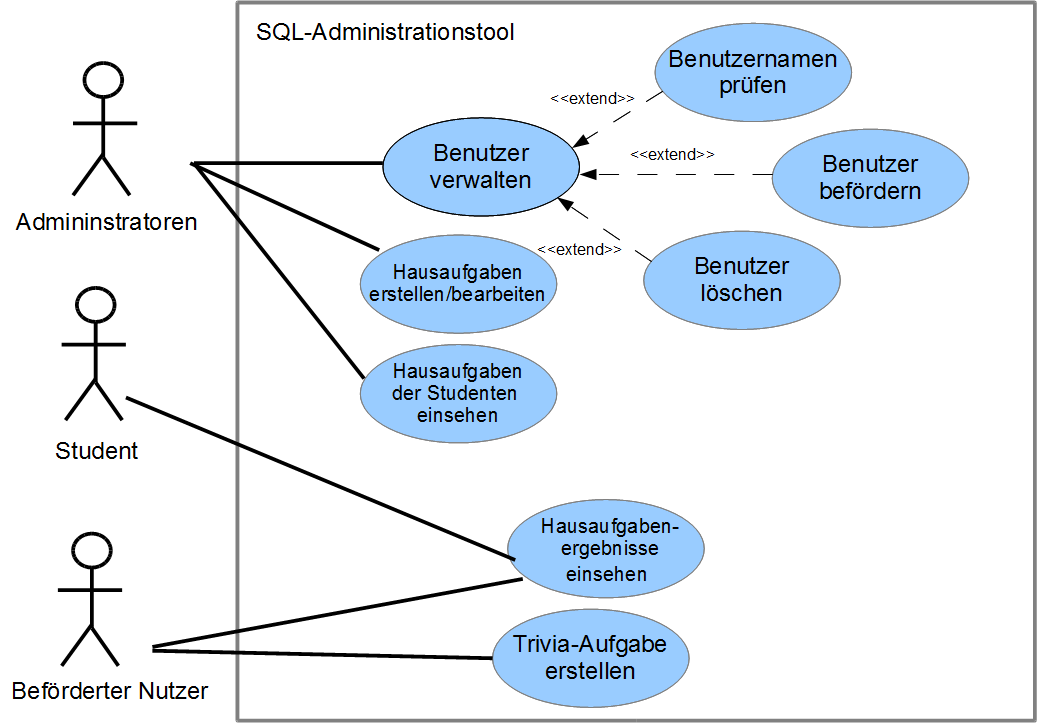
\includegraphics[width=0.8\textwidth]{figures/Admintool.PNG}
\caption{Das Admintool}
\end{figure}\\
In diesem Use-Case-Diagramm ist zu sehen, welche Möglichkeiten das Admin-Tool bereit stellt. Dabei gibt es verschiedene Nutzergruppen mit verschiedenen Rechten. 
Externe registrierte Benutzer haben standardmäßig keinen Zugriff auf das Admin-Tool.\\
Registrierte Studenten können im Admin-Tool einsehen, wie sie in ihren Hausaufgaben abgeschnitten haben. Das schließt sowohl die aktuellen, als auch die voran gegangenen ein.
Beförderte Benutzer haben, zusätzlich zu ihren Standardfunktionen (externe keine, Studenten Hausaufgaben-Übersicht) weiterhin die Möglichkeit, selber Aufgaben/ -pakete zuerstellen und die erstellten Aufgaben von anderen beförderten Benutzern zu bewerten.\\
Administratoren erhalten die Rechte zur Nutzer-, Inhalts- und Hausaufgabenverwaltung.  \\\\\\\\\\





\section{Der Story-Mode}
Das folgende Aktivit\"atsdiagramm zeigt detailliert den Ablauf der Story. Um die Story zu spielen loggt sich der User ein und w\"ahlt im Hauptmen\"u den Reiter
\glqq Story\grqq~aus. An diesem Punkt hat er bereits die M\"oglichkeit sich umzuentscheiden. M\"ochte er tats\"achlich die Story spielen, so gelangt man in das 
so genannte Laboratory, w\"ahlt ein Rezept bzw. Scroll aus und braut sich seinen gew\"unschten Trank, indem er via SQL -Statement die daf\"ur gebrauchten 
Materialien aus dem Schrank \glqq Secreterry\grqq~anfordert.
Anschlie{\ss}end hat er die M\"oglichkeit entweder aus dem Story-Modus rauszugehen oder das Minispiel im Dungeon zu starten. Dort muss er alle  H\"urden 
\"uberwinden und kann sich dann dazu entscheiden den Prozess des Trankbrauens zu wiederholen oder den Modus zu verlassen.
\begin{figure}[ht]
\centering
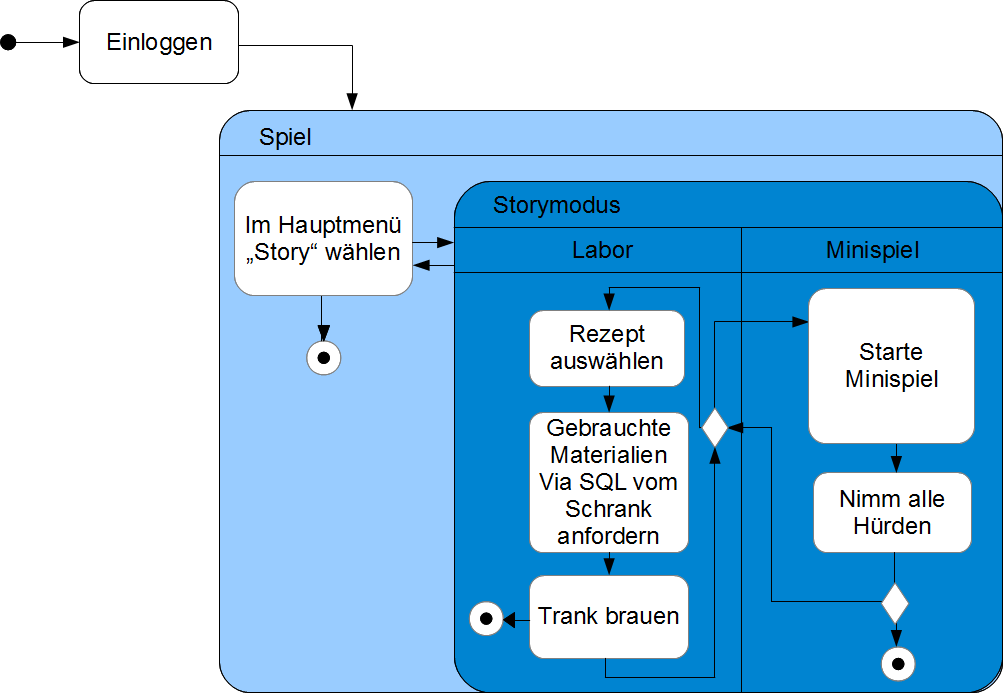
\includegraphics[width=1\textwidth]{figures/story_mode_activ.PNG}
\caption{Spielablauf im Story-Modus}
\end{figure}





\section{Das Spiel}
Im folgenden Aktivit\"atsdiagramm ist der Vorgang des Logins und der Registration beschrieben.
Nach dem Spielstart ist der Login-Bildschirm zusehen. 
Ist der Nutzer noch nicht registriert kann er dies, nach Druck auf den \glqq Sign up\grqq~Knopf, tun.
Hier muss er, je nach dem ob er Student ist oder nicht, entweder seine y-Nummer, das dazugeh\"orige Passwort, oder eine E-Mail-Adresse und ein selbst ausgedachtes 
Passwort angeben. Dazu geh\"ort in beiden F\"allen noch ein Benutzername. Nach erfolgreicher Registrierung wird man in das Hauptmen\"u weitergeleitet.\\
Sind E-Mail-Adresse, bzw. y-Nummer, und Passwort schon registriert, kann man diese im Login-Bildschirm angeben und gelang danach ins Hauptmen\"u. Der 
Benutzername wird f\"ur den Login-Vorgang nicht ben\"otigt.
\begin{figure}[ht]
\centering
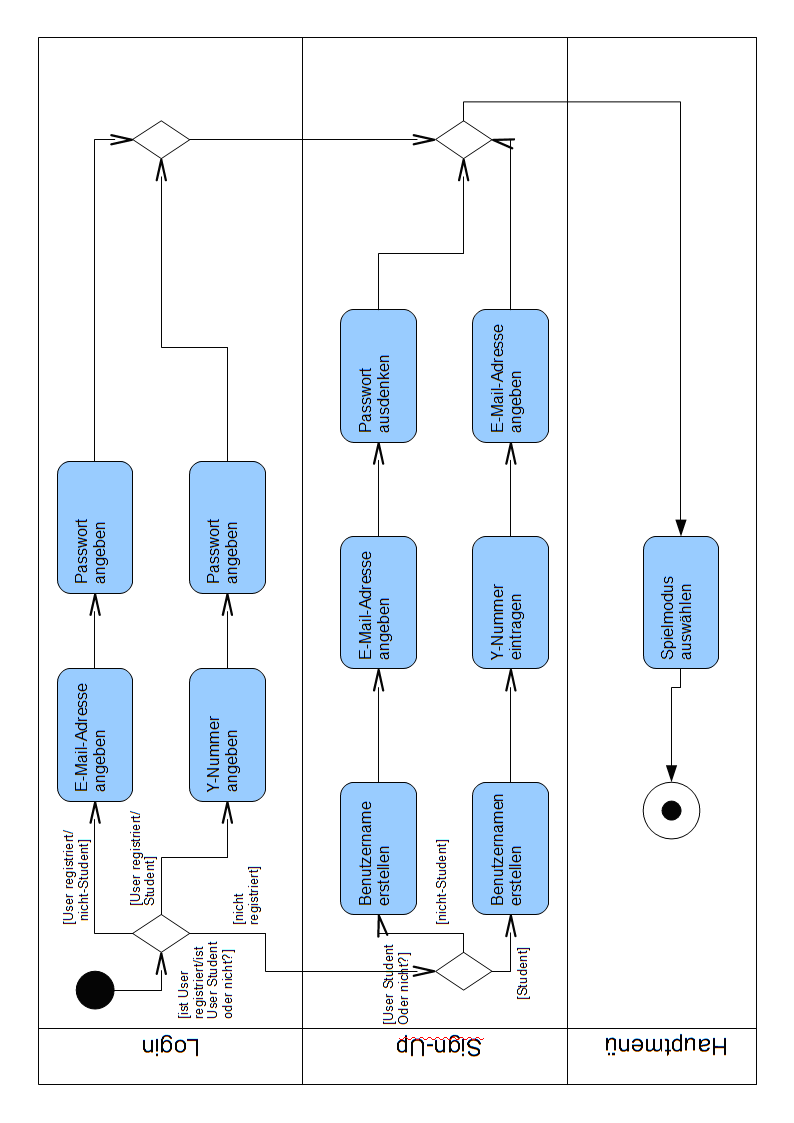
\includegraphics[width=1\textwidth]{figures/aktiv_RegLog.PNG}
\caption{Login-/Registrationsvorgang}
\end{figure}


\begin{figure}[ht]
\centering
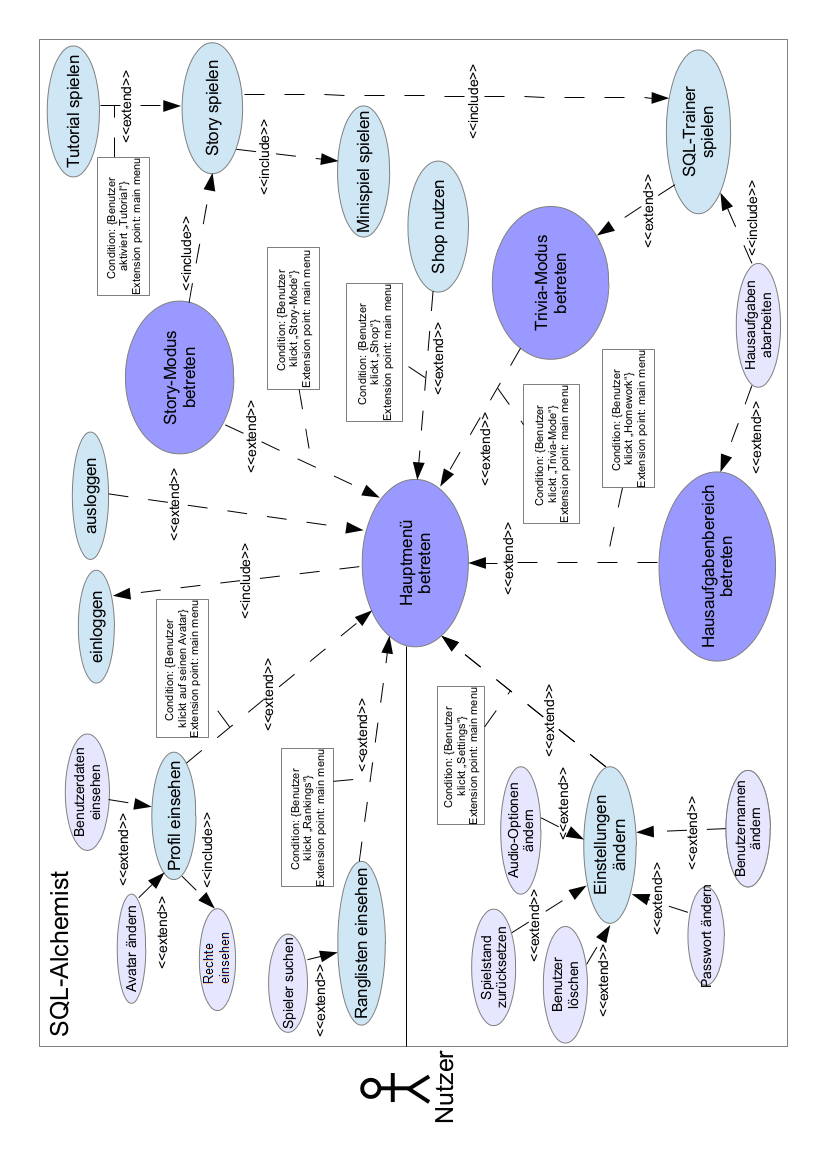
\includegraphics[width=1\textwidth]{figures/UseCaseDiagrammFinal.PNG}
\caption{Der Großteil des eigentlichen Spiels}
\end{figure}
Das folgende Use-Case-Diagramm  zeigt den Gro{\ss}teil des Spielablaufs. Loggt sich der User ein, so gelangt er in das Hauptmen\"u. In diesem Men\"u 
hat er verschiedene M\"oglichkeiten zu interagieren. Zum einen kann er sein Profil einsehen. Dort hat er die Option sowohl seinen Avatar zu \"andern, als auch seine 
Benutzerdaten einzusehen. M\"ochte der User wissen welche Nutzerrechte er hat, so kann er dies ebenfalls dort tun.
Zum anderen kann der User unterschiedliche Ranglisten einsehen, andere Spieler suchen und sich deren Rang anzeigen lassen.

Eine weitere M\"oglichkeit in dem Men\"u voranzuschreiten, ist die, pers\"onliche Einstellungen zu ver\"andern. Diese sind: 
\begin{itemize}
	\item Der User kann Audio-Optionen \"andern.
	\item Er kann seinen Spielstand zur\"ucksetzen.
	\item Er hat auch die M\"oglichkeit sein Profil komplett zu l\"oschen.
	\item Er kann sein Passwort \"andern.
	\item Er kann seinen Benutzernamen l\"oschen.
\end{itemize}

Au{\ss}erdem kann der User im Shop unterschiedliche Erweiterungen f\"ur sein Spielfigur erwerben.

Des Weiteren kann der Benutzer einen von drei verschiedene Spiel-Modi w\"ahlen. Diese sind alle untereinander verkn\"upft. Betritt der Spieler den 
Hausaufgaben-Modus, so kann er dort, die von einem Wissenschaftlichen Mitarbeiter des Dozenten der Vorlesung RDB1 gestellten Aufgaben l\"osen. 
M\"ochte man diese bearbeiten, so schlie{\ss}t das die Benutzung des SQL-Trainers ein. Dieser ist ebenfalls aus dem Trivia-Modus erreichbar. Der Trainer
ist auch fester Bestandteil des Story-Modes. M\"ochte der User die Story spielen, so impliziert das ebenfalls das Spielen des Minispiels.
Im Story-Modus ist dabei die M\"oglichkeit gegeben, vor Start der eigentlichen Story, ein Tutorial zu absolvieren. Dieses ist hierbei aber eine freiwillige Option.

Die letzte Option die sich im Hauptmen\"u noch bietet, ist die, sich auszuloggen.



